\documentclass{book}
\usepackage{amsmath,amssymb,amsfonts}
\usepackage{natbib,graphicx}
\usepackage{fancyhdr}
\usepackage{cancel}
\usepackage{tikz}
\usepackage{pgfplots}
\usepackage{esint}
\usetikzlibrary{calc}
\usepgfplotslibrary{polar}


\pgfplotsset{compat=newest}
\pgfplotsset{every axis/.append style={
                     tick label style={font=\footnotesize},
                 }}
\begin{document}
\pagestyle{empty}
\begin{center}

\line(1,0){300}\\    %double backslash is for newline
\vspace{0.3cm}
{\Huge Fluid Dynamics}
\line(1,0){300}\\    %double backslash is for newline
\vspace{1cm}
\textbf{Himanshu Raj}\\20D180015\\Environmental Science and Engineering Department\\Indian Institute of Technology, Bombay
\\
\vspace{2cm}

\includegraphics[scale=0.5]{logo.png}
\end{center}
\newpage
{\Huge Abstract}
\vspace{0.8cm}

In this paper,firstly, I have tried to summarize all the \emph{Mathematicals} which are woven around the subject \textemdash \emph{Fluid Dynamics}. The coordinates systems-Curvilinear and Cartesian, both are really important to understand the subject. A superficial knowledge of Tensors is also needed which I will be sharing through my final-paper. In this, the baisc concepts are dealt which are crucial for understanding fluid-flow and Aerodynamic theory, like, Vortictiy, Stream Functions using Complex Analysis.

%newpage
\newpage
\tableofcontents
\pagenumbering{arabic}
\pagestyle{fancy}
\fancyhf{}
\rhead{\textemdash Himanshu Raj}
\lhead{Fluid Dynamics}
\begin{center}
\chapter{Introduction}
\end{center}
\hspace{0.5cm} Fluids are the type of spaces that cannot withstand any amount of shear force. They get deformed even on applying an infinitesimal amount of shear. Fluids are composed of billions of molecules that are continuously banging into one another. Fluids, study, is treated as a continuum of particles, rather than discrete ones, using Eulerian Approach, as we will deal with this later on. Fluids play a major and a tangible role in our day to day life \textemdash from our blood flow to the fuels emission to the cool engines in the JPL.\\
This paper begins with some of the introductory concepts of fluids and their behaviour and few "mathematicals" needed to deal its principles. We will be steping up the trivials, to catch up with the esoterics like., Vorticity, $K\acute{a}rm\acute{a}n$ Vortex, RANS Equations, Turbomachinery, Dimensional Analysis, Turbulence, Turbulence Closure Models, Large Eddy Simulations, ML for fluid mechanics, working of Air-Crafts.\\
Machine Learning can play a vital role in fluid mechanics. Consider a fluid flow as a collection of images, then using the concepts of image-processing, we can model fluid-flows.\\
Robust Principal Component Analysis(RPCA) can also be used in fluid-modelling, say, flow past a cylinder; we can remove the corrupt data and outliers to get more better decompositions.
All these topics will related to \emph{data-science} are left for the final report.
\newpage

\chapter{Fluid Kinematics}
\hspace{1.3cm}The world of kinematics is concentrated only on the motion of the object, not its cause. We can fine the location \emph{(x,y,z)} of an object at a different time \emph t if it is given at ($x_0$,$y_0$,$z_0$,$t_0$), using equations of motions and calculus.\\ But if we our trivial way of tracking the locations and times of different fluid  particles or packets, we would require supereon and an infinite amout of patience with a concentration like \emph{Arjuna}. So, mathematicians have solved this problem for us.\\
In order to deal any continuum like fluids, either we can treat the whole of it as one particle or use the filed variables of the fluid flow to study its motion. The later comes under \emph{Eulerian Approach}, which is deal just after.
\section{Lagrangian Approach}
This is just the trivial approach of tracking each and every particle constituting the flow. The trajectories can be found out easily using this method. \emph{The identities of the particle are made by specifying their initial position at a given time. The position of the particle at any other time can be found out by}
\begin{center}
\begin{equation}
\vec{S}=\vec{S(S_0,t)}
\end{equation}
\end{center}
Here, $\vec{S}$ is the position vector of a particle at time \emph{t}. In cartesian frame of reference, 
\begin{subequations}
\begin{equation}
x=x(x_0,y_0,z_0,t)
\end{equation}
\begin{equation}
y=y(x_0,y_0,z_0,t)
\end{equation}
\begin{equation}
z=z(x_0,y_0,z_0,t)
\end{equation}
\end{subequations}



\begin{subequations}
\begin{equation}
\vec{v}=\dot{\vec{S}}
\end{equation}
\begin{equation}
\vec{a}=\ddot{\vec{S}}
\end{equation}

\end{subequations}

\section{Eulerian Approach}
This approach requires the use of a Vector Field, distributed ove a laboratory frame of reference and the outputs are obtained in a probe fixed to the lab-frame. Generally, we incorporate velocity-field in this approach.
\begin{figure}[h]
\includegraphics[scale=0.5]{Eulerian_Method.png}
\caption{Eulerian Approach in a laboratory frame with a probe fixed which measures the curl of the velocity field.}
\end{figure}
The volume of study is known is \emph{Control Volume}. The fluid continuously enters and leaves the CV. So, this approach is generally termed as \emph{Open-System Approach} unlike \emph{Lagrangian Approach} which is a \emph{Closed System Approach}. Different material points are continuously streaming through the same laboratory points. When these two points coincide, the \emph{Eulerian} and \emph{Lagrangian} velocities coincides. We will attain a transcendental peace while solving problems using \emph{Eulerian Approach}.

\section{Material Derivative}
Material Derivative is a method to link \emph{Lagrangian} and \emph{Eulerian} approaches. We start with the \emph{Lagrangian} description of a fluid particle as \textemdash 
Let
$u\hat{x}+v\hat{y}+w\hat{z}$ be the velocity of any particle in our CV at time \emph{t}.\\
Now,
 \begin{center}
$u=u(x,y,z,t)$ \\
$v=v(x,y,z,t)$ \\
$w=w(x,y,z,t)$ \\
\end{center}
Then,
@ the location $(x+\Delta x,y+\Delta y,z+\Delta z,t+\Delta t)$ and time $t+\Delta t$ \textemdash 
\\
\begin{center}
$u+\Delta u=u(x+\Delta x,y+\Delta y,z+\Delta z,t+\Delta t)$
\\
$v+\Delta v=v(x+\Delta x,y+\Delta y,z+\Delta z,t+\Delta t)$
\\
$w+\Delta w=w(x+\Delta x,y+\Delta y,z+\Delta z,t+\Delta t)$
\end{center}
Expand it using Taylor Expansion \textemdash
\\
which is,
\begin{center}
$f(x+\Delta x)=f(x)+f'(x)(\Delta x)+f''(x)\frac{(\Delta x)^2}{2!}+f'''(x)\frac{(\Delta x)^3}{3!}=...$
\\

\end{center}
Therefore,
\begin{center}
$u+\Delta u=u(x,y,z,t)+\frac{\partial u}{\partial x}\Delta x+\cancelto{0}{\frac{\partial^2 u}{\partial x^2}\frac{(\Delta x)^2}{2!}}+...+\frac{\partial u}{\partial y}\Delta y+\cancelto{0}{\frac{\partial^2 u}{\partial y^2}\frac{(\Delta y)^2}{2!}}+...+\frac{\partial u}{\partial z}\Delta z+\cancelto{0}{\frac{\partial^2 u}{\partial z^2}\frac{(\Delta z)^2}{2!}}+...\frac{\partial u}{\partial t}\Delta t+\cancelto{0}{\frac{\partial^2 u}{\partial t^2}\frac{(\Delta t)^2}{2!}}+...$
\\
\vspace{0.5cm}
$or,\hspace{0.5cm}\Delta u=\frac{\partial u}{\partial x}\Delta x+\frac{\partial u}{\partial y}\Delta y+\frac{\partial u}{\partial z}\Delta z+\frac{\partial u}{\partial t}\Delta t$
\\
\vspace{0.5cm}
$or,\hspace{0.5cm}\frac{\Delta u}{\Delta t}=\frac{\partial u}{\partial x}\frac{\Delta x}{\Delta t}+\frac{\partial u}{\partial y}\frac{\Delta y}{\Delta t}+\frac{\partial u}{\partial z}\frac{\Delta y}{\Delta t}+\frac{\partial u}{\partial t}$
\\
\vspace{0.5cm}
$or,\hspace{0.5cm}\lim_{t\to0}\frac{\Delta u}{\Delta t}=\lim_{t\to0}(\frac{\partial u}{\partial x}\frac{\Delta x}{\Delta t}+\frac{\partial u}{\partial y}\frac{\Delta y}{\Delta t}+\frac{\partial u}{\partial z}\frac{\Delta y}{\Delta t}+\frac{\partial u}{\partial t})$
\\
\vspace{0.5cm}
$Therefore,\hspace{0.5cm} \frac{Du}{Dt}=u\frac{\partial u}{\partial x}+v\frac{\partial u}{\partial y}+w\frac{\partial u}{\partial z}+\frac{\partial u}{\partial t}$
\\
\vspace{1cm}
Similarly,\hspace{0.5cm}
$\frac{Dv}{Dt}=u\frac{\partial v}{\partial x}+v\frac{\partial v}{\partial y}+w\frac{\partial v}{\partial z}+\frac{\partial v}{\partial t}$
\\
\vspace{1cm}
$and,\hspace{0.5cm}\frac{Dw}{Dt}=u\frac{\partial w}{\partial x}+v\frac{\partial w}{\partial y}+w\frac{\partial w}{\partial z}+\frac{\partial w}{\partial t}$

\end{center}
\vspace{0.8cm}
In vector notation, 
\begin{center}
$\vec{a}=\frac{D\vec{V}}{Dt}=\frac{\partial \vec{V}}{\partial t}+(\vec{V}\cdot\nabla)\vec{V}$
\end{center}
\vspace{0.5cm}
Note,\hspace{0.2cm}\emph{Here, $\vec{V}\cdot\nabla$ is not same as $\nabla\cdot \vec{V}$, i.e., div$\vec{V}$}.
\vspace{0.5cm}
In general, \emph{Material Derivative} for any Vector or scalar field is 
\begin{center}
\begin{equation}
\frac{D()}{Dt}=\frac{\partial ( )}{\partial t}+(\vec{V}\cdot\nabla)( )
\end{equation}
\end{center}
\vspace{0.5cm}
Material derivative is also known as \emph{Substantial Derivative}.
\newpage
\emph{\textbf{{Illustration}}
\\
The velocity field is of the form
\begin{center}
$\vec{V}(x,y)=g(y)\hat{x}+f(x)\hat{y}$
\end{center}
and the density varies in a reactor as $\rho(x,y)=\rho_0\exp(-x^2-y^2)$. Find the rate of change of density at $(x_0,y_0)$ and at origin(let it be at the center of the reactor).}
\\
\vspace{0.1cm}
\\
As, Material derivative is-\hspace{0.2cm}
$\frac{D()}{Dt}=\frac{\partial ( )}{\partial t}+(\vec{V}\cdot\nabla)( )$. So rate of change of density is given by\textemdash
\\


\begin{equation*}
\begin{split}
\frac{D(\rho)}{Dt}&=\frac{\partial ( \rho)}{\partial t}+(\vec{V}\cdot\nabla)(\rho)\\
&=(\vec{V}\cdot\nabla)(\rho)\\
&=g(y)\frac{\partial \rho}{\partial x}+f(x)\frac{\partial \rho}{\partial y}+\\
&=-2\rho(xg(y)+yf(x))
\end{split}
\end{equation*}
$\therefore$\hspace{0.2cm}at the origin, material derivative is $0$ and at $(x_0,y_0,z_0)$, it can be intuitively said as, the curve of $\rho$ flattens out at the origin, and hence its derivative vanishes out to zero. 
\\
\vspace{1cm}
\begin{center}
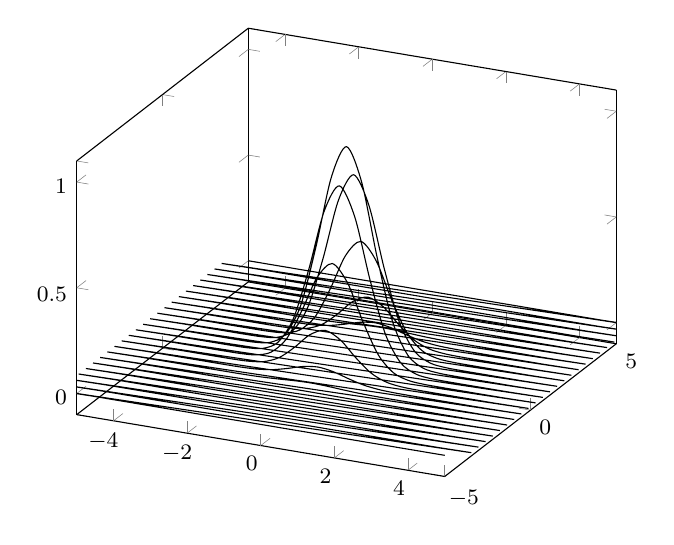
\begin{tikzpicture}
\begin{axis}
\addplot3[surf,smooth]{exp(-x^2-y^2)};
\end{axis}
\end{tikzpicture}
\end{center}
\section{Acceleration in curvilinear coordinate system}
\subsection{In Polar Coordinate System}
\begin{equation*}
\begin{split}
\vec{r}&=r(cos(\theta)\hat{x}+sin(\theta)\hat{y})\\
\hat{r}&=cos(\theta)\hat{x}+sin(\theta)\hat{y}\\
\hat{\theta}&=-sin(\theta)\hat{x}+cos(\theta)\hat{y}\\
and,MD=\frac{D(\vec{V})}{Dt}&=\frac{\partial \vec{V}}{\partial t}+(\vec{V}\cdot\nabla)(\vec{V})\\but\\
\frac{D\vec{V}}{Dt}&=\frac{\partial \vec{V}}{\partial t}\frac{dt}{dt}+\frac{\partial \vec{V}}{\partial r}\frac{dr}{dt}+\frac{\partial \vec{V}}{\partial \theta}\frac{d\theta}{dt}
\end{split}
\end{equation*}
as we know that, $\vec{V}=V_r\hat{r}+V_\theta\hat{\theta}$\\
\begin{equation*}
\begin{split}
\frac{\partial \vec{V}}{\partial r}\frac{dr}{dt}&=V_r\frac{\partial (V_r\hat{r}+V_\theta\hat{\theta})}{\partial r}\\
&=V_r(\hat{r}\frac{\partial V_r}{\partial r}+V_r\frac{\partial \hat{r}}{\partial r}+\hat{\theta}\frac{\partial V_\theta}{\partial r}+V_\theta\frac{\partial \hat{\theta}}{\partial r})\\
&=V_r(\hat{r}\frac{\partial V_r}{\partial r}+\hat{\theta}\frac{\partial V_\theta}{\partial r})\\
\vspace{0.3cm}
\frac{\partial \vec{V}}{\partial \theta}\frac{d\theta}{dt}&=\frac{V_\theta}{r}(\frac{\partial  (V_r\hat{r}+V_\theta\hat{\theta})}{\theta} \\
&=\frac{V_\theta}{r}(V_r\frac{\partial \hat{r}}{\partial \theta}+\hat{r}\frac{\partial V_r}{\partial \theta}+V_\theta\frac{\partial \hat{\theta}}{\partial \theta}+\hat{\theta}\frac{\partial V_\theta}{\partial \theta})\\
&=\frac{V_\theta}{r}(V_r\hat{\theta}+\hat{r}\frac{\partial V_r}{\partial \theta}+V_\theta(-\hat{r})+\hat{\theta}\frac{\partial V_\theta}{\partial \theta})
\\
\therefore\hspace{0.3cm}\frac{D\vec{V}}{Dt}&=\frac{\partial \vec{V}}{\partial t}+(V_r\frac{\partial V_r}{\partial r}+\frac{V_\theta}{r}\frac{\partial V_r}{\partial \theta}-\frac{V_\theta^2}{r})\hat{r}+(V_r\frac{\partial V_\theta}{\partial r}+\frac{V_\theta V_r}{r}+\frac{V_\theta}{r}\frac{\partial V_\theta}{\partial \theta})\hat{\theta}
\end{split}
\end{equation*}
\\
\subsection{In Cylindrical Coordinate system}
\begin{equation*}
\begin{split}
\vec{\rho}&=r(cos(\theta)\hat{x}+sin(\theta)\hat{y})+z\hat{z}\\
\hat{r}&=cos(\theta)\hat{x}+sin(\theta)\hat{y}\\
\hat{\theta}&=-sin(\theta)\hat{x}+cos(\theta)\hat{y}\\
\hat{z}&=\vec{k}\\
\vspace{0.2cm}\vec{V}(r,\theta,z,t)&=V_r\hat{r}+V_\theta\hat{\theta}+V_z\hat{z}
\\
\end{split}
\end{equation*}
as\begin{equation*}
\begin{split} MD=\frac{D\vec{V}}{Dt}&=\frac{\partial \vec{V}}{\partial t}\frac{dt}{dt}+\frac{\partial \vec{V}}{\partial r}\frac{dr}{dt}+\frac{\partial \vec{V}}{\partial \theta}\frac{d\theta}{dt}+\frac{\partial \vec{V}}{\partial z}\frac{dz}{dt}\\
\therefore\hspace{0.3cm}\frac{\partial\vec{V}}{\partial r}\frac{dr}{dt}&=V_r(\frac{\partial (V_r\hat{r}+V_\theta\hat{\theta}+V_z\hat{z})}{\partial r})\\
&=V_r(\frac{\partial V_r}{\partial r}\hat{r}+\frac{\partial \hat{r}}{\partial r}V_r+\frac{\partial V_\theta}{\partial r}\hat{\theta}+\frac{\partial \hat{\theta}}{\partial r}V_\theta+\frac{\partial V_z}{\partial r}\hat{z})\\
&=V_r(\frac{\partial V_r}{\partial r}\hat{r}+0+\frac{\partial V_\theta}{\partial r}\hat{\theta}+0+\frac{\partial V_z}{\partial r}\hat{z})\\
&=V_r(\frac{\partial V_r}{\partial r}\hat{r}+\frac{\partial V_\theta}{\partial r}\hat{\theta}+\frac{\partial V_z}{\partial r}\hat{z})\\
and, \frac{\partial\vec{V}}{\partial \theta}\frac{d\theta}{dt}&=\dot{\theta}(\frac{\partial V_r}{\partial \theta}\hat{r}+V_r\frac{\partial \hat{r}}{\partial \theta}+\hat{\theta}\frac{\partial V_\theta}{\partial \theta}+V_\theta\frac{\partial \hat{\theta}}{\partial \theta}+\frac{\partial V_z}{\partial \theta}\hat{z})\\
&=\frac{V_\theta}{r}(\frac{\partial V_r}{\partial \theta}\hat{r}+V_r\hat{\theta}+\frac{\partial V_\theta}{\partial \theta}\hat{\theta}-V_\theta\hat{r}+\frac{\partial V_\theta}{\partial z}\hat{z})\\
also,  \frac{\partial\vec{V}}{\partial z}\frac{dz}{dt}&=V_z(\frac{\partial V_r}{\partial z}\hat{r}+\frac{\partial V_\theta}{\partial z}\hat{\theta}+\frac{\partial V_z }{\partial z}\hat{z})\\
\therefore\hspace{0.3cm}\frac{D\vec{V}}{Dt}&=\frac{\partial \vec{V}}{\partial t}+(V_r\frac{\partial V_r}{\partial r}+\frac{V_\theta}{r}\frac{\partial V_r}{\partial \theta}-\frac{V_\theta^2}{r}+V_z\frac{\partial V_r}{\partial z})\hat{r}+(V_r\frac{\partial V_\theta}{\partial r}+\frac{V_\theta}{r}\frac{\partial V_\theta}{\partial \theta}+V_z\frac{\partial V_\theta}{\partial z}+\frac{V_r V_\theta}{r})\hat{\theta}+  \\&  (V_r\frac{\partial V_z}{\partial r}+\frac{V_\theta}{r}\frac{\partial V_z}{\partial \theta}+V_z\frac{\partial V_z}{\partial z})\hat{z}\\
\end{split}
\end{equation*}
\subsection{In Spherical Coordinate System}
Here also, we follow the same steps as above.
\begin{equation*}
\begin{split}
x&=rsin(\theta)cos(\phi)\\
y&=rsin(\theta)sin(\phi)\\
z&=rcos(\theta)\\
Also, \vec{r}&=x\hat{x}+y\hat{y}+z\hat{z}\\
\implies \vec{r}&=r(sin(\theta)cos(\phi)\hat{x}+sin(\theta)sin(\phi)\hat{y}+cos(\theta)\hat{z)}\\
\implies \hat{r}&=(sin(\theta)cos(\phi)\hat{x}+sin(\theta)sin(\phi)\hat{y}+cos(\theta)\hat{z)}\\
\vspace{0.25cm}
We\hspace{0.1cm}have,\hat{\phi}&=\frac{\frac{\partial \vec{r}}{\partial \phi}}{|\frac{\partial \vec{r}}{\partial \phi}|}\\
and,\hat{\theta}&=\frac{\frac{\partial \vec{r}}{\partial \theta}}{|\frac{\partial \vec{r}}{\partial \theta}|}\\
\end{split}
\end{equation*}
Upon solving and putting all these in matrix notation, we get-\
\\
$\begin{pmatrix}
sin(\theta)cos(\phi)  &  sin(\theta)sin(\phi)  &  cos(\theta)\\
cos(\theta)cos(\phi)  &  cos(\theta)sin(\phi)  &  -sin(\theta)\\
-sin(\phi)  &  cos(\phi)  &  0
\end{pmatrix}$
$\begin{pmatrix}
\hat{x}\\
\hat{y}\\
\hat{z}
\end{pmatrix}$
$=$
$\begin{pmatrix}
\hat{r}\\
\hat{\theta}\\
\hat{\phi}
\end{pmatrix}$
\\
\begin{equation*}
\begin{split}
\vec{V}(r,\theta,\phi)=V_r\hat{r}+V_\theta\hat{\theta}+V_\phi\hat{\phi}\\
as,MD=\frac{D\vec{V}}{Dt}&=\frac{D\vec{V}}{Dt}=\frac{\partial \vec{V}}{\partial t}\frac{dt}{dt}+\frac{\partial \vec{V}}{\partial r}\frac{dr}{dt}+\frac{\partial \vec{V}}{\partial \theta}\frac{d\theta}{dt}+\frac{\partial \vec{V}}{\partial \phi}\frac{d\phi}{dt}\\
&=V_r(\frac{\partial V_r}{\partial r}+\frac{V_\phi}{r}\frac{\partial V_r}{\partial \phi}+\frac{V_\theta}{r sin\phi}\frac{\partial V_r}{\partial \theta}-\frac{V^2_\phi+V^2_\theta}{r})\hat{r}\\&+(V_r\frac{\partial V_\phi}{\partial r}+\frac{V_\phi}{r}\frac{V_\phi}{\partial \phi}+\frac{V_\theta}{rsin\phi}\frac{\partial V_\phi}{\partial \theta}-\frac{V_r V_\phi}{r}-\frac{V^2_\theta cot\phi}{r})\hat{\phi}+\\&(V_r\frac{\partial V_\theta}{\partial r}+\frac{V_\phi}{r}\frac{\partial V_\theta}{\partial \phi}+\frac{V_\theta}{rsin\phi}\frac{\partial V_\theta}{\partial \theta}+\frac{V_\theta V_r}{r}+\frac{V_\theta V_\phi}{r})\hat{\theta}+\frac{\partial \vec{V}}{\partial t}
\end{split}
\end{equation*}\\
\newpage
\emph{\textbf{{Illustration}}\\
Figure below shows four Jet-Engines which are of different shapes. First one is a conical frustrum, then an exponentially decreasing shape, a circular one and a parabolic. Compare the acceleration of the gas near the nozzle. Consider the flow to be steady.}\\
\begin{figure}[h]
\includegraphics[scale=0.4]{linera_jet.png}
\includegraphics[scale=0.5]{expo_jet.png}
\includegraphics[scale=0.3]{circular_jet.png}
\includegraphics[scale=0.4]{parabolic_jet.png}
\caption{Jet-engine outer-casing whose diameter varies with distance.}
\end{figure}\\
In all the above cases, by symmetry, the net change in velocity is only observed in the axial direction.\\
For linear,we have, $D(x)=D_i-\frac{(D_i-D_0)}{L}x$ so, $A(x)=\frac{\pi D(x)^2}{4}$.\\
$\therefore $
\begin{equation*}
\begin{split}
u&=\frac{4Q}{\pi (D_i-\frac{(D_i-D_0)}{L}x)^2}\\
as,a_x&=u\frac{du}{dt}\\
\therefore,\vspace{0.1cm}a_x&=u\frac{8Q(D_o-D_i)}{\pi D_x^3}\\
\implies a_x&=\frac{32Q^2(D_o-D_i)}{\pi^2 D_x^5}
\end{split}
\end{equation*}
In the case of exponentially decreasing one, since the curve in 3d is just a surface of revolution around the x-axis whose generating curve is $y=e^{-x}$ . \\
\begin{equation*}
\begin{split}
y^2+z^2&=[r(x)]^2=e^{(-2x)}\\  %don't forget the curly braces
R(x)&=e^{-x}\\
and, u&=\frac{Q}{\pi e^{-2x}}\\
\therefore a_x&=u\frac{du}{dt}\\
\implies a_x&=\frac{2Q^2 e^{4x}}{\pi^2}\\
\end{split}
\end{equation*}
Next, we have the circular one, whose acceleration with x is found out to be $\frac{2Q^2x}{\pi^2 (a^2-x^2)^3}$ and for the parabolic one, it is $\frac{Q^2}{\pi^2 (a-x)^3}$.
\begin{center}
\begin{tikzpicture}
\begin{axis}[title=a v/s x for ]
\addplot[smooth]{3/(2-3*x)};
\end{axis}
\end{tikzpicture}
\end{center}
\begin{center}
\begin{tikzpicture}
\begin{axis}
\addplot[smooth]{5*exp(2*x)};
\end{axis}
\end{tikzpicture}
\end{center}
\begin{center}
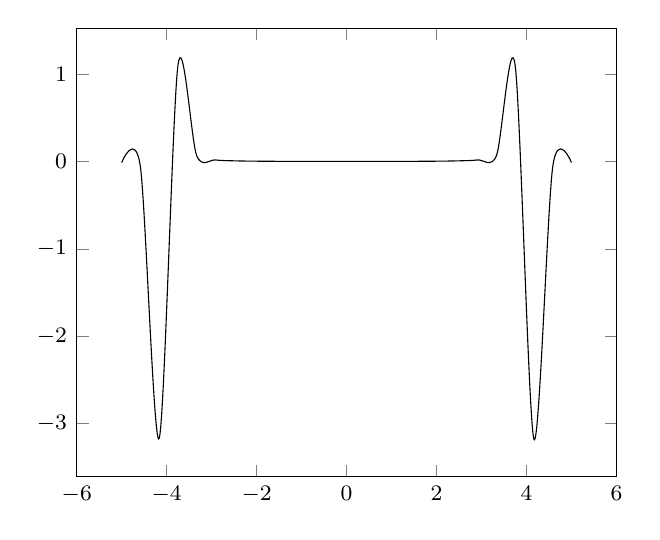
\begin{tikzpicture}
\begin{axis}
\addplot[smooth]{8/(16-x^2)^3};
\end{axis}
\end{tikzpicture}
\end{center}
\begin{center}
\begin{tikzpicture}
\begin{axis}
\addplot[smooth]{8/(4-x)^3};
\end{axis}
\end{tikzpicture}
\end{center}

\section{Rotation of fluids}
Rotation simply means change in orientation. If an object doesn't look the same during the course of its motion, then it may be rotating, maybe it has deformed while it was moving! Fluids rotate if one part of it has a velocity different than the other and rotation can be well understood by angles. We can't say that the capsules of the famous London Eye to be rotating. \\
\begin{center}
\begin{figure}[h]
\includegraphics[scale=0.4]{irrot.png}
\includegraphics[scale=0.4]{rrot.png}
\caption{Left:No rotation, only translation\\ .Right:Rotation with translation}
\end{figure}
\end{center}
When fluid rotates, it is said that a vortex is developed. From your coffee while stirring in moka pot to the famous $K\acute{a}rm\acute{a}n$ Vortex in the South Atlantic Ocean.
\\
\hspace{0.8cm}
The rotation can be well understood if we use \emph{curl} of a vector. The curl of a vector $\vec{A}$ is $\nabla \times \vec{A}$. Here, we will study the rotation using velocity vector field, $\vec{V}$, as there is no other option like a force field as in Electrodynamics and the amusing, \emph{Magnetohydrodynamics}.\\
Angular velocity, the rate of change of angular displacements, $\dot{\theta}$ is $\frac{v_\theta}{r}$. As, I  earlier said, \emph{The rotation in fluids arise because of the local differences in their velocity of flow.}However, this is not the sole reason behind rotation. \\
But, for the time-being let us assume that rotation is due to this only.\\
Consider a canonical illustration in which there are two fluid-line elements, of length $\delta x$ and $\delta y$. For the line horizontal line-element the rotation is produced by vertical component of the velocity and for the  vertical line-element the rotation is produced by horizontal component of the velocity. The line elements have relative velocities $\delta x$ and $\delta y$.
\begin{center}
\begin{tikzpicture}
\draw (0,0) -- (4,0);
\draw (0,0) -- (0,4);
\draw [-to,thick,red](4,0)--(4,1) ;
\node at (-0.2,2){$\delta y$};
\draw [-to,thick,red](0,4)--(1,4);
\node at (2,-0.2){$\delta x$};
\node at (4,1.2){$\delta v$};
\node at (1.2,4){$\delta u$};
\node at (-0.05,-0.05){A};
\node at (4.1,-0.1){B};
\node at (-0.12,4.1){C};
\end{tikzpicture}
\end{center}
\begin{equation*}
\begin{split}
\delta v&=v_B-v_A\\
&=v(x+\delta x,y)-v(x,y)\\
&=\frac{\partial v}{\partial x}\times \delta x\\
and, \frac{\delta v}{\delta x}&=\frac{\partial v}{\partial x}\\
\end{split}
\end{equation*}
\emph{Similarly,}\\
\vspace{0.8cm}
\begin{equation*}
\begin{split}
\frac{\delta u}{\delta y}&=\frac{\partial u}{\partial y}\\
\end{split}
\end{equation*}
As we know that, $\dot{\theta}=\frac{\delta v}{\delta x}-\frac{\delta u}{\delta y}$, since counterclockwise in taken as positive direction, the average rate of rotation,
\begin{equation*}
\begin{split}
 \omega_{xy}=\frac{1}{2}(\frac{\partial v}{\partial x}-\frac{\partial u}{\partial y})
\end{split}
\end{equation*}
$\omega$ is just the rotation rate. It can be global \textemdash a bulk of fluid or local \textemdash microscopic or mesoscopic portion of the fluid. Generally, the local rotation rate or spin, is governed by the term \emph{Vorticity}.
Mathematically, it is given by, 
\begin{equation}
\begin{split}
\vec{\Omega}&=\vec{\nabla}\times \vec{V}
\end{split}
\end{equation}
But, the global rotation rate is equal to the average of the individual local rotation rates. So, 
\begin{equation}
\begin{split}
\vec{\omega}&=\frac{1}{2}(\vec{\nabla}\times \vec{V})
\end{split}
\end{equation}
The direction of the vorticity vector is along the direction of $\omega$ or perpendicular to the plane of rotation of the fluid. The line which is always tangent to the vorticity vectors, is known as vortex line.\\
If we calculate the flux of vorticity vector in a plane of region, which is bounded by a curve ${\partial d}=C$, which is a positively oriented, piecewise-smooth, simple closed curve in the plane, the it is equal to the line-integral of the velocity vector around that curve. This statement is nothing but, Green's theorem of vector calculus. In 3d, this gets mould into \emph{Stokes' Theorem}.\\
Mathematically, 
\begin{equation}
\begin{split}
Circulation &=\oint_{\partial d}\vec{V}.d\vec{s} \\
&=\iint_{D}(\vec{\nabla}\times \vec{V}).d\vec{A}
\end{split}
\end{equation}
Now, if we are asked to calculate the vorticity from circulation, then we will follow these steps\textemdash Take an infinitesimal volume around that point, in which Vorticity is to be find out. Calculate the line integral around that the boundary of that volume element and divide the result by the surface-area of that region. This is a veracious result if we don't take any \emph{points of singularity} in our region.
\begin{equation*}
\begin{split}
so, \vec{\nabla}\times \vec{V}&=\lim_{A \to 0}\frac{1}{A(D)}\oint_{\partial d}\vec{V}.d\vec{s}\\
or, \vec{\nabla}\times \vec{V}&=\lim_{A \to 0}\frac{1}{A(S)}\oint_{\partial s}\vec{V}.d\vec{s}\\
\end{split}
\end{equation*}
\section{Potential Flow}
Analogous to any vector field like electric field due to static charge distribution, whose curl is identically zero, indicating their \emph{Irrotationality}, we bring out the potential into play, to understand the fluid-flow, more esoterically.
\emph{Mathematically,}\\
\begin{equation}
\begin{split}
\vec{V}&=\nabla{\varphi}\\
\end{split}
\end{equation}
In a two-dimensional fluid-flow, we can write\textemdash
\begin{equation*}
\begin{split}
\vec{V}=&\begin{bmatrix}u(x,y)\\v(x,y)\end{bmatrix}
\end{split}
\end{equation*}
Now, we define another very crucial term in the vocabulary of fluid dynamics \textemdash{Stream function $(\psi)$}. Basically, the stream function gives information about the streamlines and is equal for a streamline. In other words, $\psi$ is constant for a streamline. So, we can get the equation of a streamline by setting-up the value of $\psi$ equal to a constant, say, C. We get the family of streamlines.\\
Mathematically,\\
\begin{equation}
\begin{split}
\begin{bmatrix}u(x,y)\\v(x,y)\end{bmatrix}&=\begin{bmatrix}\frac{\partial{\psi}}{\partial y}\\{\frac{-\partial{\psi}}{\partial x}}\end{bmatrix}\\
\end{split}
\end{equation}
For an irroational fluid-flow,
\begin{equation*}
\begin{split}
\nabla\times\vec{V}&=0\\
&=\frac{\partial v}{\partial x}-\frac{\partial u}{\partial y}\\
&=0\\
and,
\nabla\times\vec{V}&=-\frac{\partial^2 \psi}{\partial x^2}-\frac{\partial^2 u}{\partial y^2}\\
&=0\\
&\implies\nabla^2{\psi}=0
\end{split}
\end{equation*}
So, if the flow is irrotational, then the stream function satisfies the \emph{Laplace's Equation}.\\
Now, if $\exists$ the gradient of the velocity field, and if the flow is incompressible, then $\varphi$ would automatically satisfy \emph{Laplace's Equation}. 
\begin{equation*}
\begin{split}
i.e.,\nabla^2{\varphi}=0\\
Also, \vec{V}=\begin{bmatrix}u(x,y)\\v(x,y)\end{bmatrix}&=\begin{bmatrix}\frac{\partial \varphi}{\partial x}\\[0.3cm]\frac{\partial \varphi}{\partial y}\end{bmatrix}=\begin{bmatrix}\frac{\partial \psi}{\partial y}\\[0.3cm]\frac{-\partial \psi}{\partial x}\end{bmatrix}
\end{split}
\end{equation*}
\emph{The functions which satisfy Laplace's Equation are known as Harmonic Functions}.
\subsection{Elementary Flows in 2-D plane(Complex Potential)}
\subsubsection{Cauchy-Riemann Conditions and Analytic Functions}
The equation $\Phi(z)=\varphi(z)+\iota\psi(z)$ represents the \emph{Complex Potential} at any point $z$ in the Argand Plane. The potentials $\varphi$ and $\psi$ are orthogonal to each other. Hence, the velocity vector is always orthogonal to the \emph{real potential}. \\
If the functions $\varphi(z)$ and $\psi(z)$ satisfy \emph{Cauchy-Riemann Conditions} then only we can represent the potential flow using \emph{Complex Potential}.
\vspace{0.2cm}
\\
\textbf{\emph{Cauchy-Riemann Condition}}
\\
\textit{Let $\Phi(z)=\varphi(z)+\iota\psi(z)$ be defined and continuous in some neighborhood of a point z and differentiable at z itself. Then, at that point, the first-order partial derivatives of u and v exist and satisfy the Cauchy-Riemann equations.}\\
\emph{Cauchy-Riemann Equations}\textemdash
\begin{equation*}
\begin{split}
 \begin{bmatrix}\frac{\partial \varphi}{\partial x}\\[0.3cm]\frac{\partial \varphi}{\partial y}\end{bmatrix}=\begin{bmatrix}\frac{\partial \psi}{\partial y}\\[0.3cm]\frac{-\partial \psi}{\partial x}\end{bmatrix}\\
\end{split}
\end{equation*}
Clearly, any of the two matrices, can represents the velocity vector. So, for the potential flow, \emph{Cauchy-Riemann Condition} is automatically satisfied. The functions involved are known as \emph{analytic functions}. \textit{E.g. $z^2,z^3,...,cos(z),sin(z), e^z, ln(z)$ (away from the origin)}. \\
\vspace{0.3cm}
\\
\subsubsection{Complex Velocity}
Let us calculate the derivative of the Potential Function $\Psi(z)$ near a known point $z_o$. We can approach this point, by two equivalent paths, viz., parallel to the real axis or parallel to the imaginary axis. From both the direction, we will obtain, an identically equal result.\textemdash\\
\begin{equation*}
\begin{split}
\frac{d\Phi}{dz}&=\lim_{\delta x\to0}\frac{\partial \Phi}{\partial x}\\
&=\frac{\partial \varphi +\iota \psi}{\partial x}\\
&=\frac{\partial \varphi}{\partial x}+\iota\frac{\partial \psi}{\partial x}\\
&=u-\iota v
\end{split}
\end{equation*}
or,if we take our step along the y-direction, we have to take it as $\iota y$.
\begin{equation*}
\begin{split}
\frac{d\Phi}{dz}&=\lim_{\delta \iota y\to0}\frac{\partial \Phi}{\partial \iota y}\\
&=\frac{\partial \varphi +\iota \psi}{\partial \iota y}\\
&=\frac{\partial \varphi}{\partial \iota y}+\iota\frac{\partial \psi}{\partial \iota y}\\
&=-\iota\frac{\partial \varphi}{\partial  y}+\frac{\partial \psi}{\partial  y}\\
&=-\iota v + u
\end{split}
\end{equation*}
It is here good to mention that, the complex potential $\Phi$ has all the information about the fluid flow. Starting right from the PDE, \emph{Laplace's Equation}, we can get the velocity vector from the Real and Imaginary parts of $\Phi$, and also, we can find out the trajectory of the any particle in the flow by the relation \textemdash
\begin{equation*}
\begin{split}
\begin{bmatrix}\dot x\\[0.3cm]\dot y\end{bmatrix}&=\begin{bmatrix}u(x,y)\\[0.3cm]v(x,y)\end{bmatrix}\\
\end{split}
\end{equation*}
\subsubsection{Power Laws}
Suppose the complex potential is given by\textemdash
\begin{equation*}
\begin{split}
\Phi(z)&=\phi(z)+\iota\psi(z)\\
and, \Phi(z)&=U_{\infty}z^n\\
\end{split}
\end{equation*}
where A is a real constant.
\begin{equation*}
\begin{split}
\Phi(z)&=U_{\infty}(re^{(\iota\theta)n})\\
\implies \phi&=U_{\infty}r^ncosn\theta \\
and, \psi&=U_{\infty}r^nsinn\theta
\end{split}
\end{equation*}
Let $\theta=\frac{\pi}{n}$. Then $n=1$ represents the trivial case of uniform flow i.e.,
\begin{equation*}
\begin{split}
\phi&=U_{\infty}x\\
and,\psi&=U_{\infty}y\\
\end{split}
\end{equation*}
This is none other than a uniform flow parallel to the x-axis.
\\
For $n=2$:
\begin{equation*}
\begin{split}
\Phi(z)&=U_{\infty}z^2\\
\implies \phi&=U_{\infty}r^2cos2\theta\\
and, \phi&=U_{\infty}r^2sin2\theta\\
or,\psi&=2U_{\infty}xy\\
So, \begin{bmatrix}u(x,y)\\v(x,y)\end{bmatrix}&=\begin{bmatrix}\frac{\partial \psi}{\partial y}\\[0.3cm]\frac{-\partial \psi}{\partial x}\end{bmatrix}=\begin{bmatrix}2U_{\infty}x\\[0.3cm]-2U_{\infty}y\end{bmatrix}
\end{split}
\end{equation*}
\begin{center}
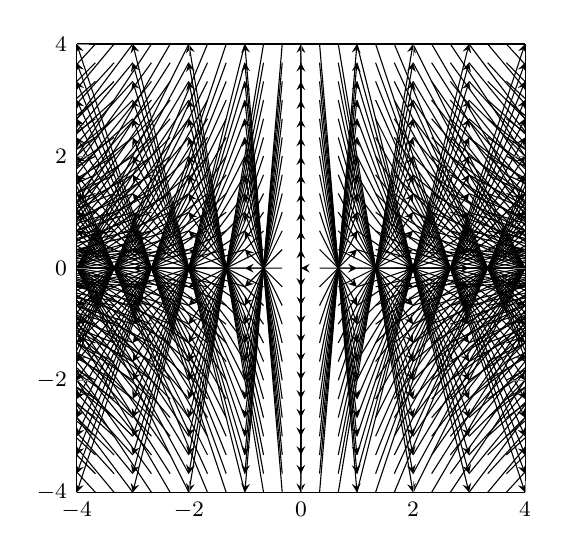
\begin{tikzpicture}
\begin{axis}[ xmin = -4, xmax = 4,
    ymin = -4, ymax = 4,
    zmin = 0, zmax = 1,
    axis equal image,
    view = {0}{90},]
\addplot3[quiver={u={2*x},v={-2*y},},-stealth,domain =-4:4,domain y=-4:4]{0};
\end{axis}
\end{tikzpicture}
\end{center} 
Clearly, we can see that the stagnation point is the origin. This can be physically interpreted as fluid-flow near two perpendicular walls. In the fig. above, the streamlines are shown. Orthogonal to the streamlines, exists the potential of velocity. \\
For $n=3$ we get a sort of a $60^o$ corner of a wall.\\
For $n=\frac{3}{2}$ we get a flow near a  $120^o$ corner of a wall. It may be observed that, the walls form an angle greater than $180^o$ for $n<1$ and an angle smaller than $180^o$ for $n>1$. Also, the corner is a stagnation point for flow in a wall angle smaller than $180^o$, and , in contrast, it is a point of infinite velocity for wall anl=gles greater than $180^o$, and the origin behaves as a singular point.\\
\subsubsection{Gyres}
Now consider a different type of flow-pattern observed in many physical phenomena, such as Ocean Mixing, Gyres etc. Let the stream-function be given as\textemdash
\begin{equation*}
\begin{split}
\psi(x,y)&=sin(\pi x)sin(\pi y)\\
\vec{V}=\begin{bmatrix}u(x,y)\\v(x,y)\end{bmatrix}&=\begin{bmatrix}\pi sin(\pi x)cos(\pi y)\\-\pi cos(\pi x)sin(\pi y)\end{bmatrix}
\end{split}
\end{equation*}
\begin{center}
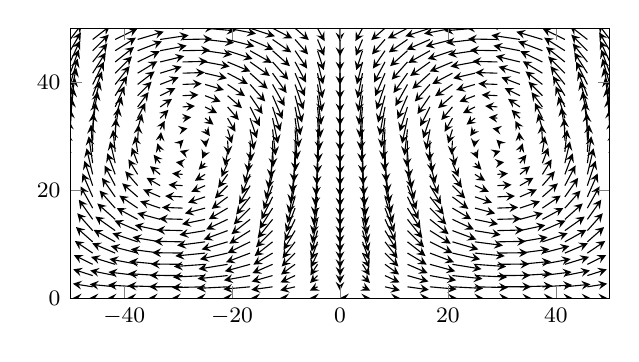
\begin{tikzpicture}
\begin{axis}[ xmin = -50, xmax = 50,
    ymin = 0, ymax = 50,
    zmin = 0, zmax = 1,
    axis equal image,
    view = {0}{90},]
\addplot3[quiver={u={2*pi*sin(pi*x)*cos(pi*y)},v={-2*pi*cos(pi*x)*sin(pi*y)},},-stealth,domain =-50:50,domain y=0:50]{0};
\end{axis}
\end{tikzpicture}
\end{center} 
Gyres are formed by the winds and geophysical circulations. \textit{In particular, the double gyre represents a typical large-scale ocean circulation phenomenon often observed in the northern mid-latitude ocean basins. This circulation is quite dominant and is persistent, consisting of sub-polar and sub-tropical gyres.}[Krishna et. al.].\\
Clearly, we can see that this vector field is rotational but divergent-free or incompressible.
\subsubsection{Rankine half-body}
This system can be thought of as the superposition of a uniform flow and a point-source. The reason behind this esoteric assumption is that, if we get the source-arrangements as mentioned, then we would get a stream-line, of a certain geometry which is identically same as the \emph{Rankine Half-Body}, the surface of which can be represented using polar coordinates as $r=\frac{q}{2\pi}\frac{\pi-\theta}{Usin\theta}$. Let, for simplicity, the flow is along the x-direction and the point-source is located at the origin, as shown below.
\begin{equation*}
\begin{split}
\varphi&=Ux+\frac{q}{2\pi}lnr\\
\psi&=Uy+\frac{q}{2\pi}\theta\\
\end{split}
\end{equation*}
The nose of the body, is the stagnation point. At this point the velocity is zero. Since, a zero vector has practically no direction, so we say that, the streamlines intersect at the stagnation point.
\begin{figure}[h]
\includegraphics[scale=0.5]{rankine_HalfBody.png}
\caption{Rankine Half-Body in 2-dimension}
\end{figure}
\subsubsection{Rankine Oval}
The Rankine oval is the superposition of a source and a sink at a distance 2a and a uniform stream as shown in the figure.
\begin{equation*}
\begin{split}
So, \psi&=U_{\infty}y-\frac{q}{2\pi}tan^{-1}{\frac{2ay}{x^2+y^2-a^2}}
\end{split}
\end{equation*}
\textbf{\textit{Illustration}}\\
\textit{Consider a 2D flow near a stagnation point. Find the complex potential, velocity vector, potential function, stream function and plot the streamlines.}\\
Let $\Phi(z)$ be the complex potential for the fluid-flow and the stagnation point be $z_o$. Using Taylor series, we can write as \textemdash\\
\begin{equation*}
\begin{split}
\Phi(z)&=\Phi(z_o)+\Phi '(z_o)(z-z_o)+\Phi ''(z_o)\frac{(z-z_o)^2}{2}+...\\
\end{split}
\end{equation*}
Now, $\Phi '(z_o)$ will be zero at the stagnation point and the h.o.t. are neglected.
\begin{equation*}
\begin{split}
\Phi(z)&=\Phi''(z_o)\frac{(z-z_o)}{2}\\
\end{split}
\end{equation*}
Let us shift our origin to the stagnation point. So, $z_o=0$. Also, let us do an esoteric substitution as, $z\rightarrow ze^{-\iota \frac{\beta}{2}}$. 
So,\\
\begin{equation*}
\begin{split}
\Phi(z)&=\frac{1}{2}z^2(ae^{\iota\beta})\\
&=z^2\\
&=\frac{a}{2}z^2\\
\end{split}
\end{equation*}
where a is any scalar.\\
Now,
\begin{equation*}
\begin{split}
as, \Phi(z)&=\frac{1}{2}(x+\iota y)^2\\
&=\frac{1}{2}a(x+iy)^2\\
&=\frac{a}{2}(x^2-y^2+2\iota x y)\\
\end{split}
\end{equation*}
So, $\phi(x,y)=\frac{a}{2}(x^2-y^2)$ and $\psi(x,y)=2axy$.\\
Interstingly, we can find the velocity vector in an other way around \textemdash
\begin{equation*}
\begin{split}
\frac{d \Phi}{dz}&=az=a(x+\iota y)\\
\therefore \begin{bmatrix}u(x,y)\\[0.3cm]v(x,y)\end{bmatrix}&=\begin{bmatrix}ax\\[0.3cm]-ay\end{bmatrix}\\
\end{split}
\end{equation*}
\\
\begin{center}
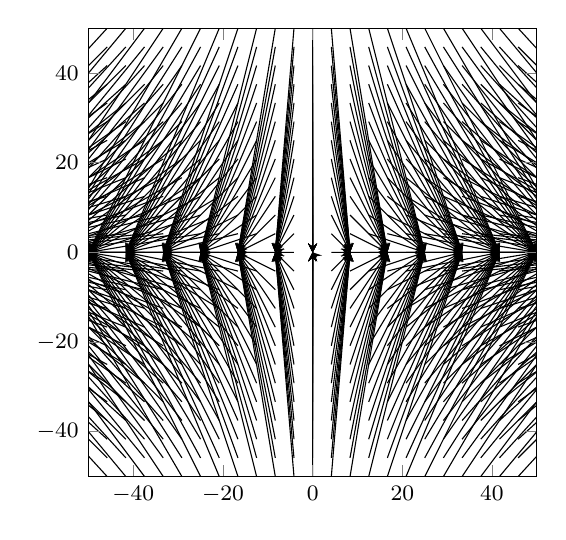
\begin{tikzpicture}
\begin{axis}[ xmin = -50, xmax = 50,
    ymin = -50, ymax = 50,
    zmin = 0, zmax = 1,
    axis equal image,
    view = {0}{90},]
\addplot3[quiver={u={x},v={-y},},-stealth,domain =-50:50,domain y=-50:50]{0};
\end{axis}
\end{tikzpicture}
\end{center} 
\section{Superposition of Elementary Flows}
This is a very powerful tool that helps up solving complex flows by breaking down into two or more simpler or elementary flows.
\subsubsection{Potential Flow past a circular cylinder}
The potential flow past a circular cylinder is equivalent to the superposition of a uniform flow at infinity and a doublet.
\begin{equation*}
\begin{split}
\Phi(z)&=U_\infty z + \frac{m}{z} \\
         &=U_\infty r^{\iota \theta}+\frac{m}{r^{\iota \theta} }\\
         &=U_\infty r({cos{\theta}+\iota sin{\theta}})  +  \frac{m}{r(cos{\theta}+\iota sin{\theta})}\\
         &=(U_\infty r+\frac{m}{r})cos{\theta} + \iota(U_\infty r- \frac{m}{r})sin{\theta} \\
\end{split}
\end{equation*}
This will generate a body of particular shape. \\
The countour of the body must be a streamline, i.e., $\psi=const$.\\
By convention, this $\psi=0$
\begin{equation*}
\begin{split}
\implies (U_\infty r- \frac{m}{r})sin{\theta} &=0 \\
\implies U_\infty r= \frac{m}{r} & or, \sin{\theta}=0 \\
\implies m=U_\infty r^2 & or, \theta=0, \pi \\
\end{split}
\end{equation*}
Now, we have got the radius of the cylinder i.e., $R=\sqrt{\frac{m}{U_\infty}}$. \\
Conversely, If we take the strength of a doublet as $m=U_\infty R^2$, then we represent a particular flow which is nothing but the flow past a cylinder of radius $\sqrt{\frac{m}{U_\infty}}$. So, m is the key here. \\
Now for calculating the lift and drag force, we will follow the following procedures as given below. 
\subsubsection{Blasius Force theorem-Derivation}
Consider a general cylinder and there is potential flow around it as shown below. Since, it is an ideal fluid, so there is no viscosity.
\begin{equation*}
\begin{split}
dF_D-\iota dF_l&=-pdy-\iota pdx \\
                      &=-\iota p(dx-\iota dy) \\
                      &=-\iota pdz \\
and, \oint (dF_D-\iota dF_l)&=F_D-\iota F_l \\
                                         &=-\iota \oint p(dx-\iota dy) 
\end{split}
\end{equation*}


\begin{figure}[!h]
\includegraphics[scale=1]{wow_blasiusPDF.pdf}
\caption{Force on an arbitrary cylinder}
\end{figure}
\newpage
Using Bernouilli's Theorem, we have \textemdash
\begin{equation*}
\begin{split}
p_\infty + \frac{1}{2}\rho U_\infty ^2 &=p +\frac{1}{2}\rho v^2 \\
p_\infty + \frac{1}{2}\rho U_\infty ^2&=p + \frac{1}{2}\rho(u^2+v^2)\\
\therefore F_d-\iota F_L &= \iota \oint [\frac{1}{2}\rho (u+\iota v)(u-\iota v)-\cancelto{0}{(p_\infty + \frac{1}{2}\rho U_\infty ^2)}]dz^\ast \\
\end{split}
\end{equation*}
Now, 
\begin{equation*}
\begin{split}
(u+\iota v)(dx-\iota dy)&= udx -\iota \cancelto{0}{(udy -vdx)} +vdy\\
\end{split}
\end{equation*}
Because the countour of the body is itself a streamline.\\
Again,
\begin{equation*}
\begin{split}
F_D-\iota F_L &= \frac{\iota}{2}\oint \rho (u+\iota v)(u -\iota v)(dx-\iota dy)\\
&=\frac{\iota}{2}\oint \rho (u -\iota v)(u-\iota v)(dx +\iota dy)\\
&=\frac{\iota}{2}\rho (u-\iota v)(u-\iota v)dz\\
&=\frac{\iota}{2}\oint \rho (\frac{d\Phi}{dz})^2 dz \\
\end{split}
\end{equation*}
We know that \textemdash
\begin{equation*}
\begin{split}
\Phi(z)&=\phi+\iota \psi \\
and \frac{\Phi(z)}{dz}&=(u-\iota v)\\
\end{split}
\end{equation*}
The above equation represents the complex velocity, which can be used in the Blasius-Force Equation.
\subsubsection{Using Blasius-Force Equation to solve \textit{Flow past a circular cylinder}.}
Here, by seeing the geometry, we incorporate polar-coordinates in order to make our work simpler.
\begin{equation*}
\begin{split}
\frac{\Phi(z)}{dz}&=u-\iota v \\
&=(V_rcos\theta-V_\theta sin\theta)-\iota (V_\theta cos\theta + V_rsin\theta)\\
&=(V_r-\iota V-\theta)(cos\theta -\iota sin\theta)\\
&=(V_r-\iota V_\theta)e^{-\iota \theta}\\
\end{split}
\end{equation*}
Also, 
\begin{equation*}
\begin{split}
\frac{d\Phi}{dz}&=U_{\infty}-\frac{m}{z^2}\\
&=U_\infty-\frac{m}{r^2}e^{-2\iota \theta}\\
&=(U_\infty e^{\iota \theta}-\frac{m}{r^2}e^{-\iota \theta})e^{-\iota \theta}\\
&=[U_\infty(cos\theta+\iota sin\theta)-\frac{m}{r^2}(cos\theta-\iota sin\theta)]e^{\iota \theta}\\
&=[(U_\infty-\frac{m}{r^2})cos\theta-\iota(-U_\infty-\frac{m}{r^2})sin\theta]e^{\iota \theta}\\
&=(V_r-\iota V_\theta)e^{\iota \theta}\\
\end{split}
\end{equation*}
On comparing, we get \textemdash
\begin{equation*}
\begin{split}
V_r&=(U_\infty-\frac{m}{r^2})cos\theta \\
and,V_\theta&=(-U_\infty-\frac{m}{r^2})sin\theta
\end{split}
\end{equation*}
Now, we use \textbf{Residue Theorem} \textemdash
\begin{equation*}
\begin{split}
\oint \frac{d\Phi}{dz} dz &= 2\pi \iota (\Sigma_{Residues})
\end{split}
\end{equation*}
and, $f(z)=\frac{d\Phi}{dz}$ can be expressed by Laurent Series as \textemdash
\begin{equation*}
\begin{split}
f(z)&=...+\frac{C_{-2}}{z^2}+\frac{C_{-1}}{z}+C_o+C_1 z+C_2 z^2...\\
\end{split}
\end{equation*}
In all the practical applications, we mainly focus in these four terms. \\
Here, $C_{-2}$ represents the flux through the cylinder, which is obviously zero. $C_{-1}$ represents Circulation, which is also zero here. $C_o$ for free-streem velocity.\\
Using Residue Theorem, we get \textemdash
\begin{equation*}
\begin{split}
\oint(1+\frac{1}{z^4}-\frac{2}{z^2})dz&=0+\oint \frac{1}{z^4}dz-\cancelto{0}{2\oint\frac{1}{z^2}}\\
&=\oint \frac{\iota r e^{\iota \theta}}{r^4 e^{\iota 4 \theta}}d\theta\\
&=0\\
\end{split}
\end{equation*}
Note: Here we've used a simpler model in order to understand the theory, clearly.\\
We have got, both the lift and drag forces as zero. But, in reality this doen't happen. Lift force will be zero somehow, because of symmetry. But the vanishment of the drag force can't be ignored. We have arrived to this result because we've ignored the viscous effects and the boundary-layer concept.\\
This is known as \textbf{The D'Alembert's Paradox}.
\chapter{A qualitative discussion onTurbulent Flow}
The random or chaotic motion of fluid particles, when the inertial forces are considerably larger than the viscous forces. Turbulent motion consists of swirls and vortices \textemdash \textbf{Eddies}. \\

\begin{figure}[h]
 \includegraphics[scale=2]{leoVinci.jpg}
\caption{Leo Vinci Model of turnulence in his painting}
\end{figure}

Characteristics of turbulent flows are \textemdash
\begin{itemize}
\item Randomness of the velocity $ \vec{u}$  w.r.t. $t$.
\item Randomness of the velocity $\vec{u}$ w.r.t. $\vec{x}$ (space).
\item Intermittency is a hall-mark feature of Turbulence.
\item They may contain coherent structures, as in, $K\acute{a}rm\acute{a}n$ Vortex street.
\item It is a multi-scale phenomena.
\item Enhanced mixing and diffusion.
\item Energy Dissipation.
\item Contains \textit{Eddies} of different length-scales.
\end{itemize}

\section{Energy Cascading}
 Eddies have rotational kinetic energy. Largest eddy ($\sim$ system length scale or problem domain geometry or $\mathcal{O}(1) $ scale. Direction of flow of energy:Mean flow to Large eddy to smaller eddies.  For large eddy, Inertial forces $>$ Viscous forces. Energy will fianlly reach to the smaller eddies. \\
As the eddies becomes smaller and smaller, the viscous forces becomes more and more stronger. Because Re decreases and a stage comes when viscous forcess become equally important as the Inertial Forces. This seems more natural to me. Firstly, from a physicist point of view, every system wants to decrease its energy, by any hook or crook.\\
Secondly, and more interesting way, in terms of Hyperbolic Geometry, the system must decrease its size to fit in Euclidian Space, in which we live, just as the fractals of a tree. \\
\begin{center}
\begin{figure}[h]
\includegraphics[scale=0.68]{energy_cascading.pdf}
\caption{Energy Cascading}
\end{figure}
\end{center}
Turbulence is a multi-scale phenomena. It contains a wide range of scale, varying from an order of few mm to few meters and may be more. Ever noticed the turbulent-disastarous scene in hollywood movies, the more you zoom in \textemdash the more you see.
\begin{center}
\begin{tabular}{||c c||} 
 \hline
Largest Eddy & Smallest Eddy\\ [0.5ex] 
 \hline\hline
 $l$ & $\eta$  \\ 
 \hline
 $u_o$ & $v$  \\
 \hline
 $t$ & $t\prime$ \\
 \hline
 $\pi$ & $\epsilon$  \\
 \hline
 $\frac{u_o^3}{l}$ & $\epsilon$  \\ [1ex] 
 \hline
\end{tabular}
\end{center}
\vspace{5cm}
\textbf{References} \textemdash \\

Advance Fluid Mechanics \textemdash W.P. Graebel

\end{document}